\documentclass[conference]{IEEEtran}
\IEEEoverridecommandlockouts
\usepackage[ngerman]{babel}
% The preceding line is only needed to identify funding in the first footnote. If that is unneeded, please comment it out.
\usepackage{cite}
\usepackage{amsmath,amssymb,amsfonts}
\usepackage{algorithmic}
\usepackage{graphicx}
\usepackage{textcomp}
\usepackage{xcolor}
\usepackage{setspace}
\usepackage{booktabs}
\usepackage[export]{adjustbox}
\def\BibTeX{{\rm B\kern-.05em{\sc i\kern-.025em b}\kern-.08em
    T\kern-.1667em\lower.7ex\hbox{E}\kern-.125emX}}
\begin{document}

\title{Currency Exchange, eine App zur Anzeige von Wechselkursen mit Hilfe eines Webscrapers}


\author{\IEEEauthorblockN{1\textsuperscript{st} Matz, Annika}
\IEEEauthorblockA{\textit{dept. name of organization (of Aff.)} \\
\textit{name of organization (of Aff.)}\\
Berlin, Deutschland \\
s\_matz22@stud.hwr-berlin.de}
\and
\IEEEauthorblockN{2\textsuperscript{nd} Liebenberg, Benjamin}
\IEEEauthorblockA{\textit{dept. name of organization (of Aff.)} \\
\textit{name of organization (of Aff.)}\\
Oranienburg, Deutschland \\
s\_liebenberg22@stud.hwr-berlin.de}
\and
\IEEEauthorblockN{3\textsuperscript{rd} Reetz, Tobias}
\IEEEauthorblockA{\textit{dept. name of organization (of Aff.)} \\
\textit{name of organization (of Aff.)}\\
Berlin, Deutschland \\
s\_reetz22@stud.hwr-berlin.de}
%Beispiel wie es aussah
%\and
%\IEEEauthorblockN{3\textsuperscript{rd} Given Name Surname}
%\IEEEauthorblockA{\textit{dept. name of organization (of Aff.)} \\
%	\textit{name of organization (of Aff.)}\\
%	City, Country \\
%	email address or ORCID}
}

\maketitle


\section{Einführung}
Innerhalb unseres dualen Studiums der Informatik an der "Hochschule für Wirtschaft und Recht", nahmen wir an dem Modul Software-Engineering 2 teil. Ziel dieses ist die Entwicklung von Software, vermittelt zu bekommen und das erlernte Wissen direkt anwenden zu können innerhalb einer Projektarbeit. Dabei wird auf die Grundlagen des Projektmanagments geachtet, wofür z.B. UML-Diagrammen angefertigt werden. Zur Dokumentation des Projektes wird dieses Paper angefertigt. 
Innerhalb des Moduls werden auch Softskills gefördert, z.B. die Präsentationsfähigkeiten oder die Sozialkompetenz innerhalb von Gruppenarbeiten.

\section{Idee des Projektes}
Ein sehr großer Teil unseres Lebens dreht sich um das erwerben von unterschiedlichen Materiellen Gütern. Für unserer Arbeit werden wir vergütet, im Supermarkt kaufen wir davon unser Abendessen und an den Wochenenden und im Urlaub gehen wir auf Reisen. Auf diesen müssen wir uns in einer fremden Kultur zu Recht finden und konsumieren weiter Güter. Doch wie können wir einen Wert von diesen einschätzen, wenn wir die Währung nicht kennen? Und genau dieses Problem löst unsere App "Currency Exchange". Einfaches nachschlagen von tagesaktuellen Wechselkursen und umrechnen zwischen verschiedenen Währungen. Ein besonderes Feature ist das Umwandeln des eingegebenen Wertes in die Anzahl von Döner, welche damit gekauft werden könnten in Euro. \\\\
Die  Android-App arbeitet mit Hilfe eines Webscrapers, welcher Wechselkurse erhält.
% und Beträge der unterschied- lichen Währungen ineinander umrechnet.

\section{Projektorganisation}
Innerhalb eines Softwareentwicklungsprojekts erhalten die einzelnen Bearbeitenden verschiedene Rollen, die ihnen unterschiedliche Aufgaben zu teilen. In diesem Fall bestand das Entwicklungsteam aus wenigen Personen, so wurden keine expliziten Arbeitsbereiche vergeben.  So wurden Aufgaben nach und nach vergeben, wobei jeder Bereich eine eigene Ansprechperson besaß. Unterteilt wurde in Projektleitung, Serveradministration, Design und Testdurchführung. Zu Anfang wurde für essentiell wichtige Themen, wie z.B. die Software-Architektur oder den groben Design-Entwurf, wurden Teammeetings durchgeführt und die Umsetzung so zusammen geplant. Sichergestellt wurde so, dass jedes Teammitglied mit einbezogen wird und alle auf dem gleichen Stand sind. \\\\
Die Programmierung der Software wurde von Teammeeting zu Teammeeting aufgeteilt. Hauptsächlich kümmerten sich Benjamin und Tobias Reetz um die Programmierung des Webscrapers, sowie die Schnittstelle und ein Teil des Backend der App. Annika Matz kümmert sich vor allem um die Umsetzung des Designentwurfs zu einem funktionierenden Frontend, sowie ein Teil der Programmierung des Backend.

\subsection{Projektleitung}
Der Projektleitung wurde von Annika Matz übernommen. Unteranderem behielt sie die unterschiedlichen Abgabetermine im Blick. Außerdem sorgte sie für regelmäßig Treffen in der Gruppe und leitete diese an. Bei diesen wurde der aktuelle Stand ausgewertet, weitere Entwicklungsschritte besprochen und Aufgaben verteilt. \\\\
Des weiteren achtete sie auch auf die Projektanforderungen und führte die Qualitätssicherung durch, wodurch sie für eine angemessene Feedback innerhalb der Teammeetings sorgt.

\subsection{Serveradministration}
Der Bereich Serveradministration wurde von Benjamin Liebenberg beaufsichtigt. Aufgrund seiner weitreichenden Erfahrung in diesem Gebiet, konnte er diesen Bereich übernehmen. Er hostet unseren Webscraper auf seinem Server, sorgt für täglich aktualisierte Daten innerhalb der App und stellt die Schnittstelle für unsere App bereit.

\subsection{Design \& Testplanung}
Das Design und die Testplanung wurden zum größten Teil von Tobias Reetz übernommen. Aufgrund seiner Designerfahrung im Modul Software-Engineering 1, übernahm er diese Rolle und designte vor allem das App-Logo. Er sorgte für eine angemessene Farbgebung und dafür, dass die App aufgrund ihrer Gestaltung schnell wieder erkennt werden kann. \\\\
Außerdem übernahm er das Konkretisieren von Usability-Tests, welche wir zuvor im Plemnum entworfen hatte und führte diese mit unseren Kommilitonen durch. Damit trug er einen entscheidenen Beitrag zur Fehlersuche und somit zur Qualität unseres Programmes bei.

\section{Anforderungen}
An eine Software werden immer unterschiedliche Erwartungen und Anforderungen gestellt. Eine genaue Definition sind wichtig für den Erfolg des Projektes. In diesem Projekt werden die unterschiedlichen Anforderung in drei Kategorien unterteilt. Sie beinhalten nicht funktionale, funktionale und optionale funktionale Anforderungen.

\subsection{Nicht funktionale Anforderungen}
Nicht-funktionale Tests decken alle Anforderungen ab, welche das gesamte System ansich betreffen. Es werden somit keine Funktionen abgeprüft, sondern Eigenschaften und Bestandteile. Für das Projekt wurde besonders auf eine sehr gute Usability geachtet, was besonders durch eine intuitive und einfache Benutzung begründet werden soll.
Desweiteren soll eine Verfügbarkeit des Projekt auf Android-Handys garantiert werden. Um einen hohen Datenschutz garantieren zu können erheben wir keine Daten und speichern auch nicht die in der Vergangenheit getätigten Eingaben dem Nutzer zur Verfügung. 

\subsection{Funktionale Anforderungen}
Funktionale Anforderung definieren die Funktionen und Erwartungen der Software, welche für ein erfolgreiches Projekt erfüllt werden müssen. \\\\
Das wichtigste Ziel für die Software ist eine lauffähige Android-Handy-Applikation, welche verschiedene Eingaben zwischen verschiedenen Währungen richtig Umrechnen kann. Es soll immer ein tagesaktueller Wechselkurs bereit stehen. In die App sollen auch mindestens sieben Währungen eingebunden werden.

\subsection{Optionale funktionale Anforderungen}
Anforderungen, welche nicht essentiell notwendig für die grundlegenden Funktionsweise sind, aber sie diese erweitern, werden zu den optionalen funktionalen Anforderungen gezählt. \\\\
Zu diesen zählt die Umrechnung der Anzahl an Döner, die die Nutzenden sich mit dem eingetragenen Wert kaufen könnten in Euro. Außerdem könnte die App durch eine Funktion zum Hinzufügen von Prozentualen Werten ergänzt werden. Diese könnten zum Beispiel zur Berechnung der Mehrwertsteuer oder des Trinkgeldes genutzt werden.

\section{Entwurf}
Innerhalb eines Entwurfs wird der Aufbau und die Struktur des Projektes geplant und fest gehalten. Dieser besteht in diesem Projekt aus zwei der Systemarchitektur, einem Sequenzdiagramm und dem groben Designentwurf. Nach diesen Vorgaben wurde die App entwickelt.

\subsection{Systemarchitektur}
Eine Systemarchitektur beschreibt die Struktur des Projektes, so wie alle seine vorkommenden Bereiche und wie diese miteinander interagieren. 

\begin{figure}[h]
	\centering
	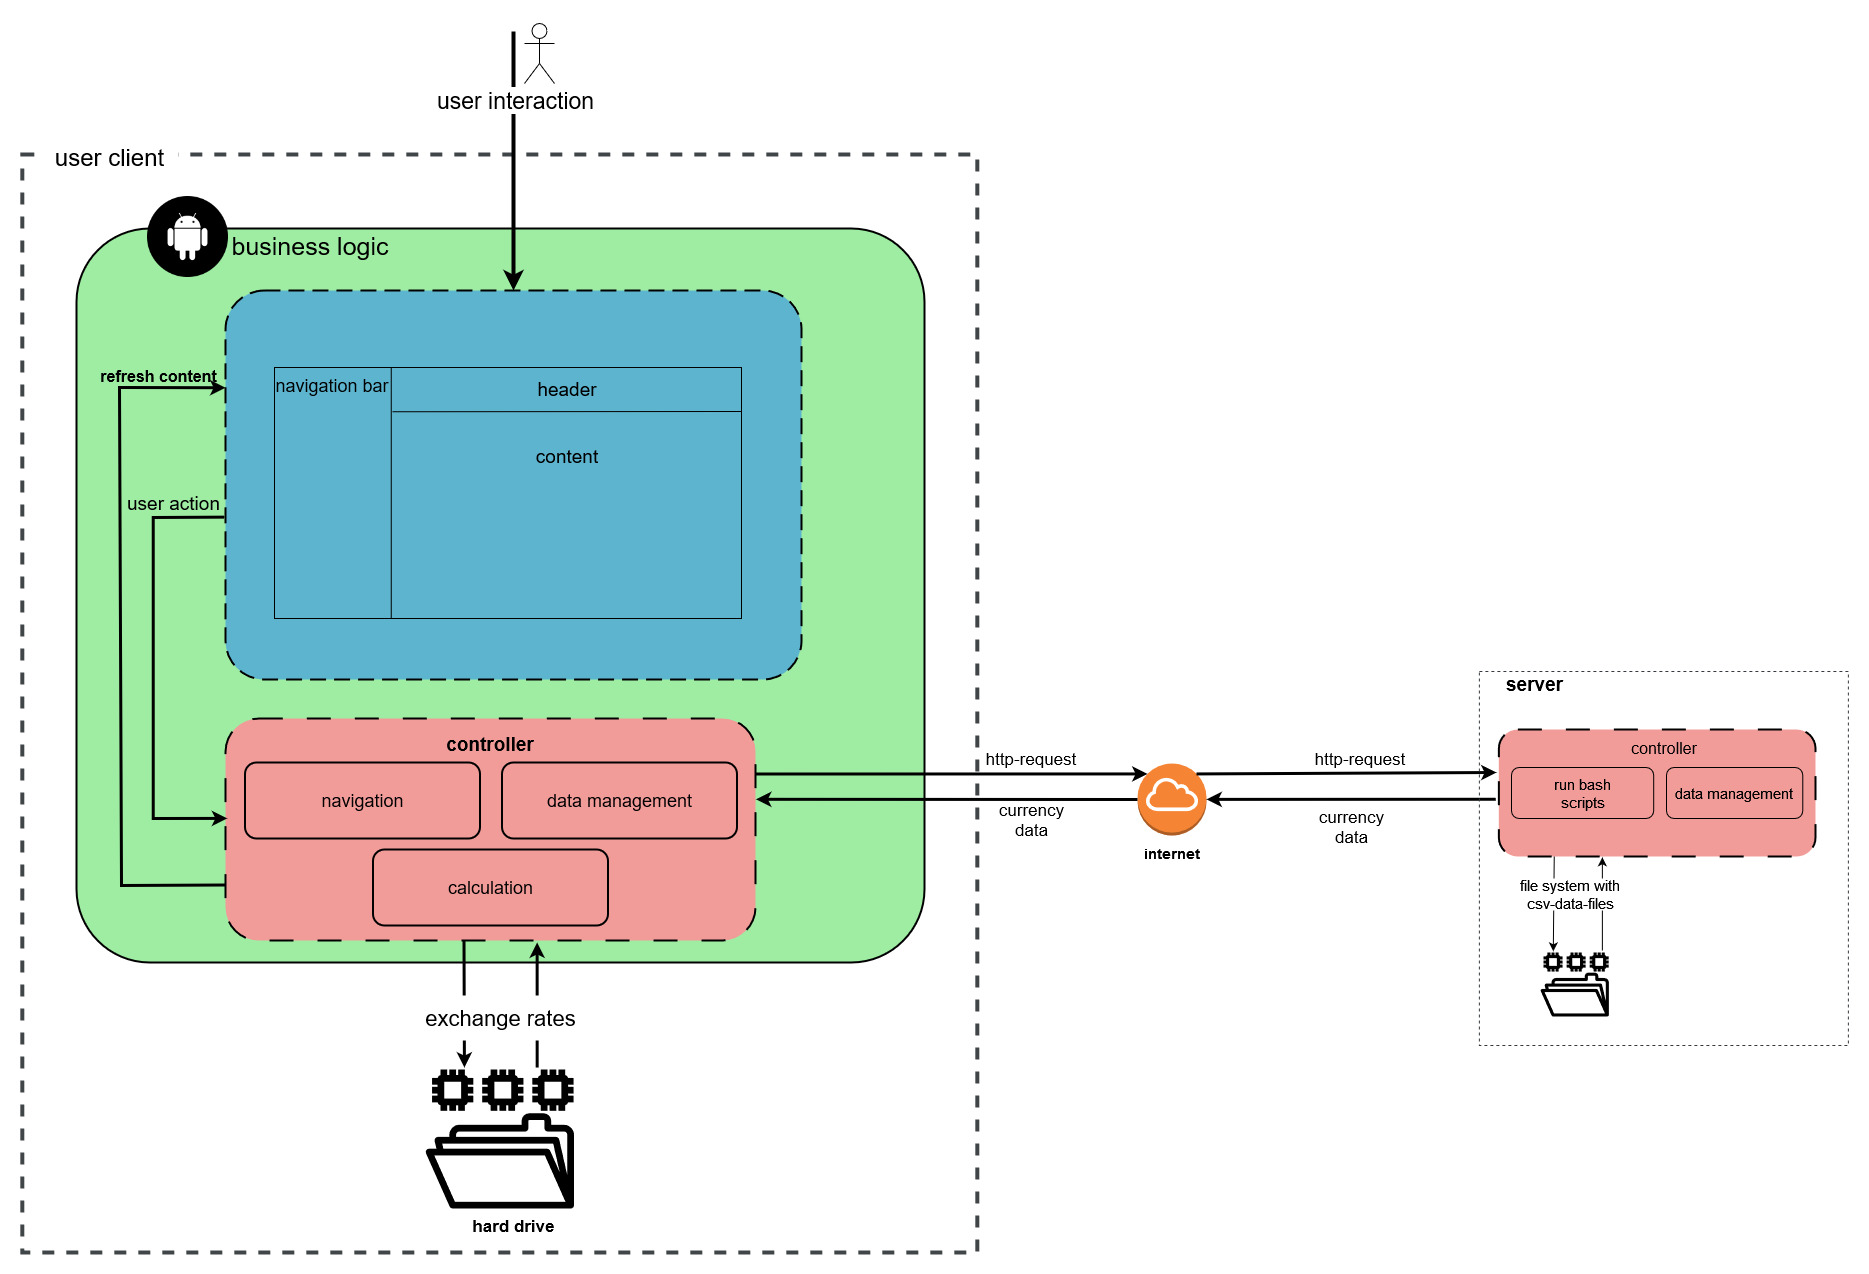
\includegraphics[width=1\linewidth, frame]{Software-Architektur_SWEII}
	\caption[Softwarearchitektur]{Softwarearchitektur}
	\label{fig:software-architektursweii}
\end{figure}
\noindent
Abbildung \ref{fig:software-architektursweii} zeigt wie die Softwarearchitektur strukturiert ist. Auf der linken Seite ist der User-Client abgebildet und auf der Rechten der Server. Aufgrund dieser zwei Komponenten, handelt es sich um eine Zwei-Tier-Architektur. \\\\
Im User-Client ist zusehen, dass der User mit der in blau gekennzeichneten Benutzeroberfläche interagiert. Diese besteht aus einem Header, einer Navigationsleiste, und dem Inhalt. Über die Interaktion können Nutzende verschiedene Funktionen erreichen, diese sind als Controller im roten Bereich zu sehen sind. Diese werden in drei unterschiedliche Bereiche kategorisieren, dem Navigator, der Data-Manager und der Calculator. Der Data-Manager ist dafür zuständig die Daten in einem Ordner zu speichern und sie den Anderen Funktionen bereit zu stellen. Er stellt auch Anfragen per HTTP-Request an den Server und sorgt somit für eine aktuelle CSV-Datei mit den benötigten Wechselkursen. Der Calculator berechnet die Wechselkurse und der Navigator sortiert Daten und stellt sie der Benutzeroberfläche bereit. \\\\
 Der Controller des Servers stellt Bash-Skripte bereit, die den Webscraper täglich starten. Der Data-Manager ist hier auch wieder für die Aufarbeitung der Daten zuständig. Dabei sorgt er für die korrekte Speicherung in eine CSV-Datei.\\\\
Durch die Einbindung des Webscraper auf einem externen Server, wird eine geringe Anfrage auf die Website mit den Wechselkursen garantiert. Denn sollten zu viele Anfragen an die Webseite geschickt werden, kann es zu einer Überlastung dieser kommen. Mögliche folgen wären das Abstürzen dieser Seite.

\subsection{Sequenzdiagramm}
Das Sequenzdiagramm beschreibt die Kommunikation der unterschiedlichen Instanzen miteinander innerhalb der Software. 

\begin{figure}[h]
	\centering
	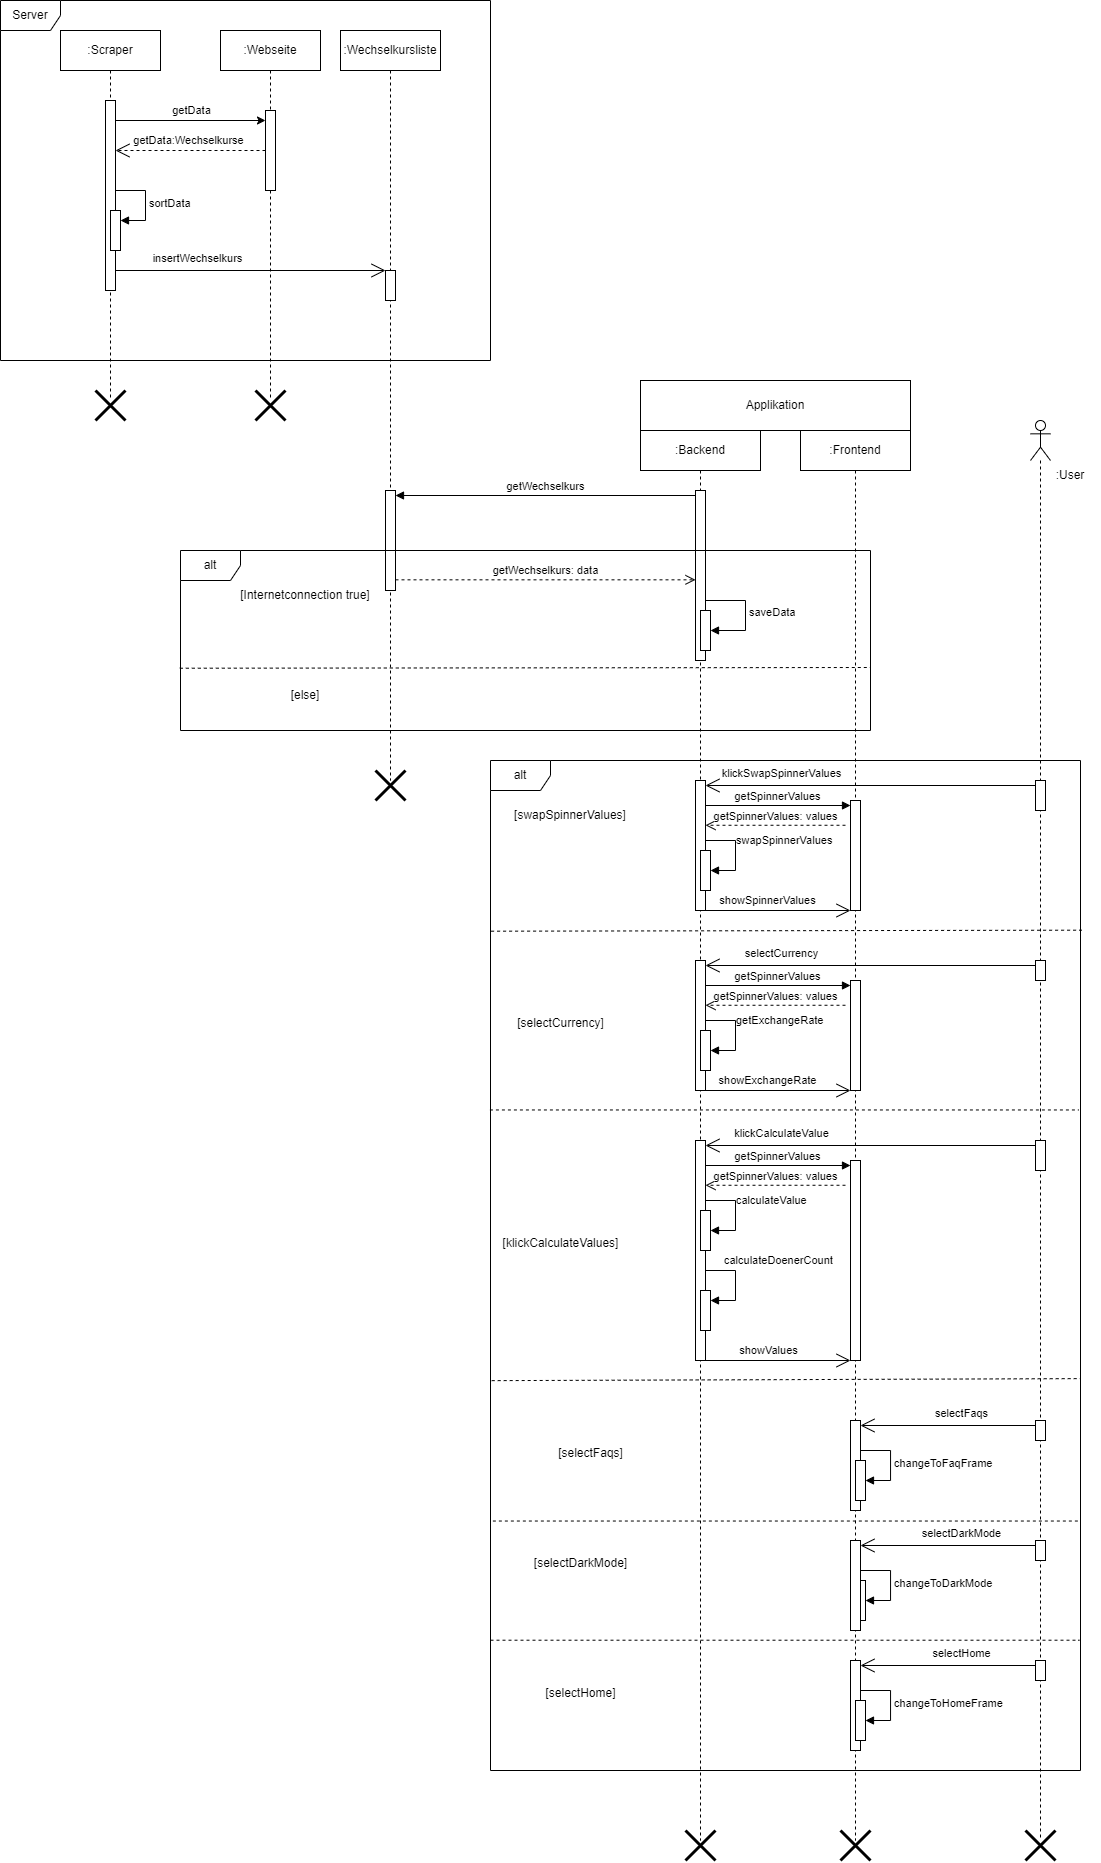
\includegraphics[width=1\linewidth, frame]{Sequenzdiagramm.drawio}
	\caption[Sequenzdiagramm]{Sequenzdiagramm}
	\label{fig:sequenzdiagramm}
\end{figure}

\noindent
Abbildung \ref{fig:sequenzdiagramm} zeigt die Gestaltung des Projektes auf. Oben links ist der Serverbereich abgebildet. Dabei holt sich der Webscraper die Daten von einer fest definierten Webseite. Danach werden diese strukturiert, alphabetisch sortiert und dann in einer CSV-Datei gespeichert. Nachfolgend ist die Applikation dargestellt. Diese ist in ein Front und Backend eingeteilt. \\\\
Das Backend schickt eine Anfrage an den Server um die aktuelle CSV-Datei zu erhalten. Jedoch nur wenn eine Verbindung zum Internet existiert, erhält er diese auch und kann sie speichern. Sollte keine Verbindung aufgebaut werden können, so wir die zu letzt aktualisierte CSV-Datei genutzt. \\\\
Innerhalb der Applikation kann der User unterschiedliche Funktionen auswählen. Die ersten drei abgebildeten Optionen haben eine ähnliche Struktur. Die nutzende Person schickt eine Anfrage an das Backend. Dieses holt sich dann die eingegebenen Daten aus dem Frontend. Wenn nun die Werte getauscht werden sollen, tauscht das Backend die Werte und übermittelt die neun dem Frontend. Wird jedoch stattdessen eine neue Währung gewählt, so wird der neue Wechselkurs im Backend berechnet und anschließend im Frontend verändert. Soll eine Umrechnung stattfinden wird zuerst der Betrag in die ausgewählte Währung übergeben und nachfolgend die Anzahl der Döner berechnet. Auch diese neuen Werte werden dann über das Frontend dem Nutzer angezeigt. \\\\
Zum Wechseln der Seite auf die Home-Seite bzw. der FAQ-Seite und zum Wechseln in den Dark-Mode bzw. Light-Mode navigiert der User sich durchs Frontend.

\section{Implementierung}

\subsection{Konsistenz}

\subsection{Vorbereitung}

\subsubsection{Versionsverwaltung}

\subsubsection{Namenskonvention}

\subsubsection{Entwicklungsumgebung und Programmiersprachen}



\section{Integration}
%Top-Down Integration
Die Integration in der Softwareentwicklung beschäftigt sich mit den Schnittstellen zwischen den verschiedensten Systemen. Teilweise werden auch Anschlüsse unter verschiedenen Funktionseinheiten benötigt. Da die App im Vergleich zu anderen Softwareprodukten eher klein ist, werden hier nicht so viele Schnittstellen benötigt. \\\\ Die erste Anbindung befindet sich zwischen dem User-Client und dem Server. Sie dient zur Transferierung von Daten. \\\\ Die zweite und letzte Schnittstelle liegt zwischen dem Server und der Webseite. Sie ist auch wie die erste Anbindung für den Transfer von Daten zuständig. \\\\ Anbindungen von verschiedenen Funktionen werden in diesem Softwareprojekt nicht benötigt, weil sie alle in dem User-Client implementiert worden sind.

\section{Tests}

\subsection{Experience-based Testing}

\subsection{Beta Tests}
Die Testung der App wurde am 13.03.2024 mit Hilfe von User-Tests durchgeführt. Bei User-Tests testen Anwender die Software und beantworten anschließend Fragen über diese. Bei den Fragen an den User wurde auf zwei unterschiedliche Bereiche gezielt Fragen gestellt. Einmal der Funktionalität der Funktionen und Sonstiges.

\subsubsection{Black-Box Test}
Die Fragen über die Funktionalitäten beschäftigten sich gezielt mit den Funktionen, wie zum Beispiel ob der Dark-Mode eingeschaltet werden könne oder Werte geändert, getauscht und umgerechnet werden können. \\\\ Bei den Fragen über die Funktionalitäten stellte sich heraus, dass die meisten Funktionen grundlegend funktionierten, allerdings Bugs enthielten. Die Währungen konnten alle ausgewählt werden. Wurde jedoch zweimal die gleiche Währung ausgewählt und in sich umgerechnet erfolgte ein Systemabsturz der App. Ein Systemabsturz entstand auch wenn als Betrag "."\space eingegeben wurde. Der Punkt dient als Kommata. Der Dark-Mode verursachte auf der FAQ-Seite auch zu Problemen, da wenn er dort eingeschaltet oder ausgeschaltet wurde, entstand auch wieder ein Systemabsturz. Ein weiterer Absturz wurde verursacht, wenn von der FAQ-Seite zu der Home-Seite gewechselt worden ist und der Dark-Mode-Knopf nicht als erstes betätigt worden ist.

\subsubsection{Usability Test}
Die sonstigen Fragen beschäftigten sich mit dem Aussehen der App und Verbesserungsvorschlägen. \\\\ Dies ergab, dass die App ein gutes Design aufweist und einfach zu verstehen ist. Ein Verbesserungsvorschlag der häufiger erwähnt worden ist, ist dass die Auswahl der Währungen doch besser zu gestalten wäre, da diese alphabetisch nach den Ländern sortiert wurden.

\section{Wartung}
Die Wartung der Anwendung wird in zwei Bereiche geteilt. Ein Bereich ist die Wartung des Servers und der andere ist von der App.

\subsection{Wartung Server}
Der Server wurde von der Firma STRATO als Service as a Infrstucture angemietet, daher wird die Wartung des Servers von STRATO übernommen.

\subsection{Wartung App}
Sobald die App fertig gestellt worden ist wird keine Wartung dieser mehr benötigt.

\section{Rollout}
Nach der Fertigstellung der App, wird eine APK für Android-Systeme erstellt. Diese APK muss dann auf dem Handy der nutzenden Person ausgeführt werden. Hierfür gibt es diverse Möglichkeiten, von denen zwei vorgestellt werden. 

\subsection{Installation über eine Direktverbindung zum PC}
Das Handy wird per Kabel mit dem Computer verbunden. Nach dem dies geschehen ist, muss die APK von dem PC irgendwo auf dem Handy gespeichert werden. Danach muss die APK nur noch per Klick auf dem Handy ausgeführt werden und die Installation von Currency Exchange erfolgt von selbst.

\subsection{Installation über den USB-Stick}
Es wird eine USB-Stick an den Computer angeschlossen. Danach wird die APK auf dem USB-Stick gespeichert und er kann dann vom Computer getrennt werden. Daraufhin wird der USB-Stick an das Handy angeschlossen. Von dem USB-Stick wird dann die APK auf dem Handy gespeichert und nur noch ausgeführt. 

\section{Ergebnis}

\section{Abschluss}



\end{document}
